\documentclass[a4paper, 12pt]{article}

\usepackage{main}
\usepackage{amsmath}

\usepackage[linesnumbered]{algorithm2e}
\SetKwComment{Comment}{/* }{ */}
\newtheorem{theorem}{Theorem}
\usepackage{siunitx}
\usepackage{lscape}
\usepackage{hologo}
\usepackage{listings}
\usepackage{hyperref}
\usepackage{pgfplots}
\usepackage{blindtext}
\usepackage{titlesec}

\usepackage{float}

\pgfplotsset{width=10cm,compat=newest}

% Table stretch
\usepackage{array}
\usepackage{xcolor}
\lstset { %
    language=C++,
    backgroundcolor=\color{black!5}, % set backgroundcolor
    basicstyle=\footnotesize,% basic font setting
}

\begin{document}

\linespread{0.5}

\title{CS165 Final Report}

\author{Lev Kruglyak}

\email{
\href{mailto:levkruglyak@college.harvard.edu}{levkruglyak@college.harvard.edu$^1$}, 
}

% Do not change the following three lines
\maketitle 
\thispagestyle{fancy} 
\pagestyle{fancy}

The goal of the project is to design and implement an optimized simple column store in C. We make several simplifying assumptions: all data stored can fit into main memory, we don't have any unexpected shutdowns or disk failures, we only need to support storing integers, etc.

\section{Milestone 1: Basic Column-Store}

In this milestone, we implement the basic functionality of a column store database server with the ability to run single-table queries. Starting with a server program that starts a UNIX socket and a simple client program which connects to the server in order to send queries, we must develop a database catalog, parsing system, and some simple single-column primitive operators.

\begin{figure}[ht]
\begin{center}
\tikzset{every picture/.style={line width=0.75pt}} %set default line width to 0.75pt
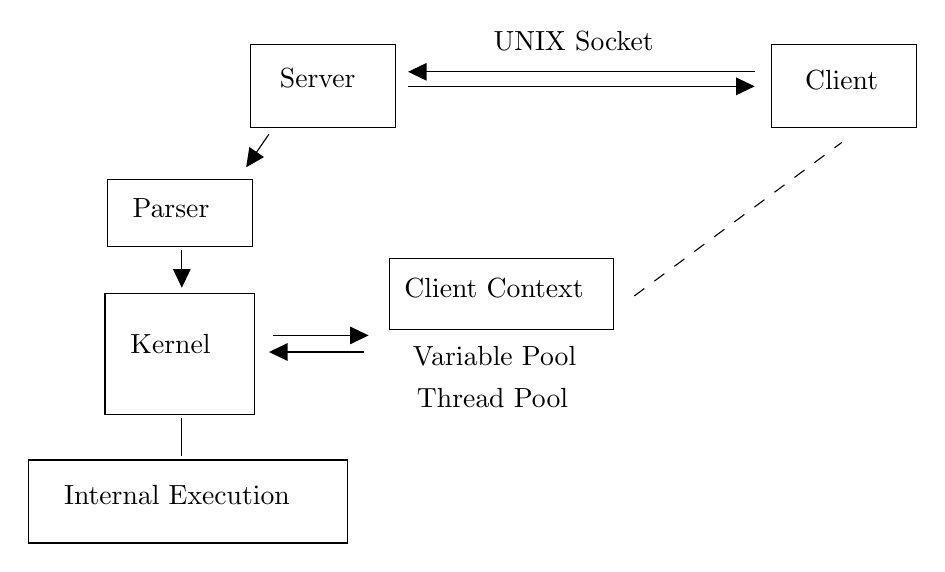
\begin{tikzpicture}[x=0.75pt,y=0.75pt,yscale=-1,xscale=1]
%uncomment if require: \path (0,300); %set diagram left start at 0, and has height of 300

%Shape: Rectangle [id:dp2683885748353101] 
\draw   (234,42) -- (304,42) -- (304,82) -- (234,82) -- cycle ;
%Shape: Rectangle [id:dp8553914278045622] 
\draw   (485,42) -- (555,42) -- (555,82) -- (485,82) -- cycle ;
%Straight Lines [id:da9276563187597906] 
\draw    (313,55) -- (477,55) ;
\draw [shift={(310,55)}, rotate = 0] [fill={rgb, 255:red, 0; green, 0; blue, 0 }  ][line width=0.08]  [draw opacity=0] (8.93,-4.29) -- (0,0) -- (8.93,4.29) -- cycle    ;
%Straight Lines [id:da2946981716802839] 
\draw    (310,62) -- (474,62) ;
\draw [shift={(477,62)}, rotate = 180] [fill={rgb, 255:red, 0; green, 0; blue, 0 }  ][line width=0.08]  [draw opacity=0] (8.93,-4.29) -- (0,0) -- (8.93,4.29) -- cycle    ;
%Shape: Rectangle [id:dp9693316726381707] 
\draw   (301,145) -- (409,145) -- (409,179) -- (301,179) -- cycle ;
%Straight Lines [id:da5012074010520422] 
\draw  [dash pattern={on 4.5pt off 4.5pt}]  (419,163) -- (519,89) ;
%Shape: Rectangle [id:dp45005500516874153] 
\draw   (165,107) -- (235,107) -- (235,139) -- (165,139) -- cycle ;
%Straight Lines [id:da83275542073072] 
\draw    (243,85) -- (233.7,98.53) ;
\draw [shift={(232,101)}, rotate = 304.51] [fill={rgb, 255:red, 0; green, 0; blue, 0 }  ][line width=0.08]  [draw opacity=0] (8.93,-4.29) -- (0,0) -- (8.93,4.29) -- cycle    ;
%Shape: Rectangle [id:dp9493274353214143] 
\draw   (164,162) -- (236,162) -- (236,220) -- (164,220) -- cycle ;
%Straight Lines [id:da1804637643032534] 
\draw    (289,190) -- (246,190) ;
\draw [shift={(243,190)}, rotate = 360] [fill={rgb, 255:red, 0; green, 0; blue, 0 }  ][line width=0.08]  [draw opacity=0] (8.93,-4.29) -- (0,0) -- (8.93,4.29) -- cycle    ;
%Straight Lines [id:da5612990729809075] 
\draw    (201,141) -- (201,156) ;
\draw [shift={(201,159)}, rotate = 270] [fill={rgb, 255:red, 0; green, 0; blue, 0 }  ][line width=0.08]  [draw opacity=0] (8.93,-4.29) -- (0,0) -- (8.93,4.29) -- cycle    ;
%Shape: Rectangle [id:dp7180700418729922] 
\draw   (127,242) -- (281,242) -- (281,282) -- (127,282) -- cycle ;
%Straight Lines [id:da1617598582069606] 
\draw    (201,222) -- (201,240) ;
%Straight Lines [id:da793423330142444] 
\draw    (288,182) -- (245,182) ;
\draw [shift={(291,182)}, rotate = 180] [fill={rgb, 255:red, 0; green, 0; blue, 0 }  ][line width=0.08]  [draw opacity=0] (8.93,-4.29) -- (0,0) -- (8.93,4.29) -- cycle    ;

% Text Node
\draw (247,52) node [anchor=north west][inner sep=0.75pt]   [align=left] {Server};
% Text Node
\draw (500,53) node [anchor=north west][inner sep=0.75pt]   [align=left] {Client};
% Text Node
\draw (350,34) node [anchor=north west][inner sep=0.75pt]   [align=left] {UNIX Socket};
% Text Node
\draw (307,153) node [anchor=north west][inner sep=0.75pt]   [align=left] {Client Context};
% Text Node
\draw (311,186) node [anchor=north west][inner sep=0.75pt]  [font=\normalsize] [align=left] {Variable Pool};
% Text Node
\draw (313,206) node [anchor=north west][inner sep=0.75pt]  [font=\normalsize] [align=left] {Thread Pool};
% Text Node
\draw (176,115) node [anchor=north west][inner sep=0.75pt]   [align=left] {Parser};
% Text Node
\draw (175,180) node [anchor=north west][inner sep=0.75pt]   [align=left] {Kernel};
% Text Node
\draw (143,253) node [anchor=north west][inner sep=0.75pt]   [align=left] {Internal Execution};
\end{tikzpicture}
\end{center}
\caption{Large scale overview of the system}
\label{fig:overview}
\end{figure}

\medskip
Now let's discuss some of the technical challenges we faced in this milestone.

\subsection{Overall Architecture}

Figure~\ref{fig:overview} shows a high level overview of the database system. One important design decision was modularity; i.e. the server and parser code doesn't touch databases, and the kernel doesn't know about the client. We also made a decision to split the kernel into an internal and external component. All of the highly performance critical code is in the internal component, and clearly marked in the code so that it can be optimized and its assembly analyzed. It also takes in very simple data types like arrays and vectors to make optimization easier. All the other custodial code is in the external shell of the kernel, and it decides whether or not to use indices for example. 

\medskip
The server has some global data such as the database tables, and some local data that is only persisted per client. The \texttt{ClientContext} structure holds this local data, which includes a variable pool for storing variables, and a thread pool for executing multithreaded operations. Each client context is destroyed when a client disconnects. The global data consists of a database object which holds tables, which hold columns. This is created when the server is first run from persisted files. Executed operators can reference either global data in the form of columns or local data in the form of variables.

\subsection{Variable Pool}

In order to quickly parse and execute queries, we need a way to efficiently look up variables that have been defined in the current session, especially for queries which could have hundreds of variables. To do this, we add a ``variable pool'' to our client context, which here just means a \texttt{char~*} to \texttt{Variable~*} hash-table. We use the \texttt{int} to \texttt{int} hash-table code for this, (see \ref{hashtable} for details and benchmarking) and replace the integer hashing function with a simple polynomial hash function. This provides excellent performance, since we already have a highly optimal hash-table implementation.

\subsection{Loading Data}

Our database can load data in the form of a csv file, with the first line corresponding to the list of columns we add data to. If the client detects a \texttt{load} instruction being passed, it enters into \texttt{CSV\_TRANSFER} mode, meaning it begins reading the file in chunks and passing them to the server.

\medskip
The first line we receive is just the table information, so we parse that and store it in the csv transfer session. The remaining data we receive consists of the vast majority of the workload. At first, we implemented a simple parsing function that used \texttt{strtok\_r} and \texttt{atoi}, which works great, but there is a lot of room for optimization.

\pgfplotstableread{load.dat}{\load}
\pgfplotstableread{load_cache.dat}{\loadt}
 \begin{figure}[ht]
     \centering
        \begin{tikzpicture}
        \begin{axis}[
            scale=0.7,
            grid = both,
            xlabel={\# of entries per colum (in millions)},
            % width = 0.5\textwidth,
            % height = 0.65\textwidth,
            ylabel={load time in ms},
            nodes near coords align={vertical},
        ]
         
        \addplot[red, very thick, mark=star] table [x = {x}, y = {fast}] {\load};
        \addplot[blue, very thick, mark=diamond*] table [x ={x}, y = {slow}] {\load};
         
        \legend{
            \texttt{FAST\_LOAD}, 
            standard load,
        }
         
        \end{axis}
        \end{tikzpicture}
        ~
        \begin{tikzpicture}
            \begin{axis}[
                scale=0.7,
                grid = both,
                xlabel={\# of entries per colum (in millions)},
                ylabel={L3 cache misses in GB},
                % width = 0.5\textwidth,
                % height = 0.65\textwidth,
                nodes near coords align={vertical},
            ]
             
            \addplot[red, very thick, mark=star] table [x = {x}, y = {fast}] {\loadt};
            \addplot[blue, very thick, mark=diamond*] table [x ={x}, y = {slow}] {\loadt};
             
            \legend{
                \texttt{FAST\_LOAD}, 
                standard load,
            }
             
            \end{axis}
            \end{tikzpicture}
        \caption{\texttt{FAST\_LOAD} performance vs standard performance}
        \label{fig:loads}
 \end{figure}

\medskip
The database system can also optionally do a \texttt{FAST\_LOAD}, which doesn't check for correctness or formatting but runs about $50\%$ faster. (See Figure~\ref{fig:loads}) This is accomplished by a one-pass scan of the data, so we parse, split, and push to columns in a single tight loop. To arrive at this optimal loop, we made extensive use of \texttt{perf record} to analyze the assembly and see which instructions were taking the longest. As the second graph in Figure~\ref{fig:loads} shows, while the cache performance had an impact, the massive difference in performance at large loads comes primarily from the actual assembly instructions.

For one thing, we inlined all function calls and removed any small allocations during tokenization. We also avoided repeated scans of the data by functions such as \texttt{strlen}, \texttt{atoi}, and \texttt{strtok\_t}. Finally, we made sure to order the if statements for analyzing characters in the right order to avoid branch mispredictions, and use short circuiting \texttt{||} and \texttt{\&\&} when necessary. This involved a significant amount of back and forth with the compiler and perf.

\medskip
It would also be possible to write a middle ground solution, i.e. one that checks for correctness in the tight loop, however we found it was helpful to have a highly optimized load that can be used for performance testing and debug purposes.

\subsection{Persisting Data}

Another challenge we faced was the persistence of data when the server shuts down. Whenever the server shuts down, we first record all of the database catalog information into a file. This is done by simply flattening the tree that represents the database hierarchy. Next, we use the \texttt{mmap} and \texttt{munmap} system calls to map the columns directly into memory. We have a separate data directory which contains this data.

\medskip
On startup, we do a similar thing, but we first read and parse the catalog, then \texttt{mmap} the data into a new column for each column that we parsed. A challenge we faced was making sure that we were using \texttt{mmap} in a way that didn't cost us any performance compared to \texttt{malloc} and reading the file directly. This involved reading a lot of \texttt{man} pages.

\subsection{Fast Scanning}

We were able to achieve an interesting speedup in our initial implementation of \texttt{select} operators. Initially we tested for whether or not an entry in a column satisfies a filter using the condition: \texttt{(data >= low) \&\& (data < high)} Since this condition has critical performance implications for the whole system, we tried several variants to get the best performance. The best one on average was to switch from using a short circuiting AND to a logical AND, i.e.: \texttt{(data >= low) \& (data < high)} This allows for better CPU pipelining and branch prediction performance, and this was experimentally verified using the branch misprediction CPU counter. 

\medskip
In the future, it might be interesting to use the distribution of the column data and selectivity of the filter to select between several variants of this condition; either short circuiting AND, short circuiting AND with conditions reversed, or logical AND.

\section{Milestone 2: Scan Sharing and Multiple Cores}

In this milestone, we improve the speed of our scans by adding support for batching operators together and distributing these across multiple cores. Since there are a lot of moving parts, a big challenge we faced was testing and understanding the performance implications of our code. We describe the implementation of the thread pool structure in Section~\ref{threadpool}. 

\medskip
We went beyond the goal and added support for batching fetches, reselections, combine, and aggregate operators. In doing so we build a solid framework for adding ``plugins'' for further optimizing shared scans.

\subsection{Introduction to Dependency Graphs}

To organize the operators that are supposed to be batch, we introduce two new types: \texttt{gen\_var} and \texttt{gen\_link}. A \texttt{gen\_var} or generic variable represents either a column or a standard database variable, e.g. select, fetch. A \texttt{gen\_link} represents one of the permissible operators, and links multiple generic variables to an output variable. Each generic variable references its parent link, or has a null reference if it's a column or a pre-existing variable.

\medskip
Now when \texttt{batch\_queries()} is first called on the client side, the server creates an empty \texttt{dep\_graph} structure, which consists of a list of generic variables. Every time an operation is executed, it is added to the graph. Once \texttt{batch\_execute()} is called, we execute this graph. See Figure~\ref{fig:graph} for an example of a dependency graph. There are several different ways to execute a dependency graph, we call these different execution methods \textit{heuristics}.

\begin{figure}
    \centering
    \tikzset{every picture/.style={line width=0.75pt}} %set default line width to 0.75pt        
    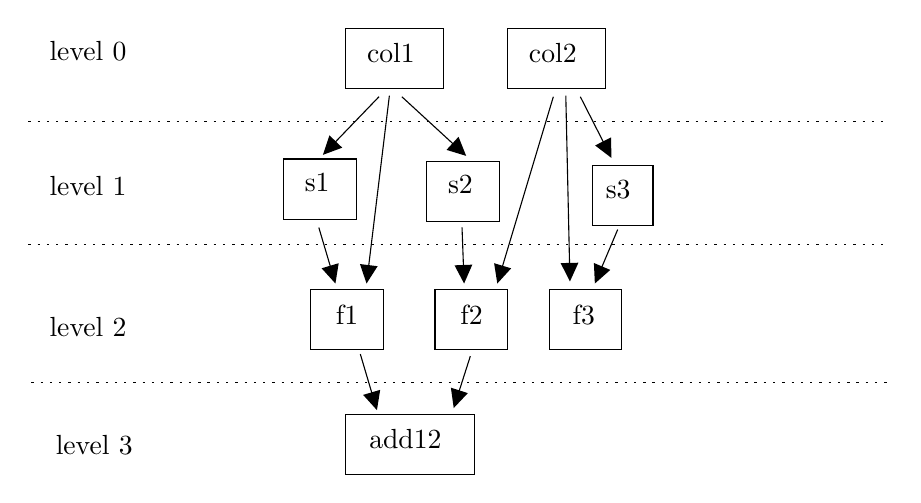
\begin{tikzpicture}[x=0.75pt,y=0.75pt,yscale=-1,xscale=1]
    %uncomment if require: \path (0,300); %set diagram left start at 0, and has height of 300
    
    %Shape: Rectangle [id:dp2683885748353101] 
    \draw   (234,42) -- (281,42) -- (281,71) -- (234,71) -- cycle ;
    %Shape: Rectangle [id:dp4334110136882279] 
    \draw   (312,42) -- (359,42) -- (359,71) -- (312,71) -- cycle ;
    
    %Shape: Rectangle [id:dp8949001820492073] 
    \draw   (204,105) -- (239,105) -- (239,134) -- (204,134) -- cycle ;
    %Shape: Rectangle [id:dp780125913097786] 
    \draw   (273,106) -- (308,106) -- (308,135) -- (273,135) -- cycle ;
    %Straight Lines [id:da0719100601557352] 
    \draw    (250,75) -- (225.08,100.84) ;
    \draw [shift={(223,103)}, rotate = 313.96] [fill={rgb, 255:red, 0; green, 0; blue, 0 }  ][line width=0.08]  [draw opacity=0] (8.93,-4.29) -- (0,0) -- (8.93,4.29) -- cycle    ;
    %Straight Lines [id:da44086937533862636] 
    \draw    (261,75) -- (289.79,101.47) ;
    \draw [shift={(292,103.5)}, rotate = 222.59] [fill={rgb, 255:red, 0; green, 0; blue, 0 }  ][line width=0.08]  [draw opacity=0] (8.93,-4.29) -- (0,0) -- (8.93,4.29) -- cycle    ;
    %Straight Lines [id:da9413600059976748] 
    \draw    (255,74.5) -- (244.36,162.02) ;
    \draw [shift={(244,165)}, rotate = 276.93] [fill={rgb, 255:red, 0; green, 0; blue, 0 }  ][line width=0.08]  [draw opacity=0] (8.93,-4.29) -- (0,0) -- (8.93,4.29) -- cycle    ;
    %Shape: Rectangle [id:dp07451665335178825] 
    \draw   (217,168) -- (252,168) -- (252,197) -- (217,197) -- cycle ;
    %Straight Lines [id:da22615066416012186] 
    \draw    (221,138) -- (228.15,162.12) ;
    \draw [shift={(229,165)}, rotate = 253.5] [fill={rgb, 255:red, 0; green, 0; blue, 0 }  ][line width=0.08]  [draw opacity=0] (8.93,-4.29) -- (0,0) -- (8.93,4.29) -- cycle    ;
    %Shape: Rectangle [id:dp2613517315309044] 
    \draw   (353,108) -- (382,108) -- (382,137) -- (353,137) -- cycle ;
    %Straight Lines [id:da33276600479540686] 
    \draw    (347,75) -- (360.64,101.83) ;
    \draw [shift={(362,104.5)}, rotate = 243.05] [fill={rgb, 255:red, 0; green, 0; blue, 0 }  ][line width=0.08]  [draw opacity=0] (8.93,-4.29) -- (0,0) -- (8.93,4.29) -- cycle    ;
    %Shape: Rectangle [id:dp8238460775644318] 
    \draw   (277,168) -- (312,168) -- (312,197) -- (277,197) -- cycle ;
    %Straight Lines [id:da01013566271222377] 
    \draw    (290,138) -- (290.89,162) ;
    \draw [shift={(291,165)}, rotate = 267.88] [fill={rgb, 255:red, 0; green, 0; blue, 0 }  ][line width=0.08]  [draw opacity=0] (8.93,-4.29) -- (0,0) -- (8.93,4.29) -- cycle    ;
    %Straight Lines [id:da015786259270902825] 
    \draw    (334,75) -- (307.86,162.13) ;
    \draw [shift={(307,165)}, rotate = 286.7] [fill={rgb, 255:red, 0; green, 0; blue, 0 }  ][line width=0.08]  [draw opacity=0] (8.93,-4.29) -- (0,0) -- (8.93,4.29) -- cycle    ;
    %Shape: Rectangle [id:dp5466424364427316] 
    \draw   (332,168) -- (367,168) -- (367,197) -- (332,197) -- cycle ;
    %Straight Lines [id:da5486348807070123] 
    \draw    (365,139) -- (355.17,162.24) ;
    \draw [shift={(354,165)}, rotate = 292.93] [fill={rgb, 255:red, 0; green, 0; blue, 0 }  ][line width=0.08]  [draw opacity=0] (8.93,-4.29) -- (0,0) -- (8.93,4.29) -- cycle    ;
    %Straight Lines [id:da5709461323740412] 
    \draw    (340,74.5) -- (341.93,161) ;
    \draw [shift={(342,164)}, rotate = 268.72] [fill={rgb, 255:red, 0; green, 0; blue, 0 }  ][line width=0.08]  [draw opacity=0] (8.93,-4.29) -- (0,0) -- (8.93,4.29) -- cycle    ;
    %Shape: Rectangle [id:dp8060256081235613] 
    \draw   (234,228) -- (296,228) -- (296,257) -- (234,257) -- cycle ;
    %Straight Lines [id:da9336176068732667] 
    \draw    (241,199) -- (248.15,223.12) ;
    \draw [shift={(249,226)}, rotate = 253.5] [fill={rgb, 255:red, 0; green, 0; blue, 0 }  ][line width=0.08]  [draw opacity=0] (8.93,-4.29) -- (0,0) -- (8.93,4.29) -- cycle    ;
    %Straight Lines [id:da5009330580253453] 
    \draw    (294,200) -- (286.91,222.14) ;
    \draw [shift={(286,225)}, rotate = 287.74] [fill={rgb, 255:red, 0; green, 0; blue, 0 }  ][line width=0.08]  [draw opacity=0] (8.93,-4.29) -- (0,0) -- (8.93,4.29) -- cycle    ;
    %Straight Lines [id:da2790068113096156] 
    \draw  [dash pattern={on 0.84pt off 2.51pt}]  (81,87) -- (496,87) ;
    %Straight Lines [id:da7828438888439926] 
    \draw  [dash pattern={on 0.84pt off 2.51pt}]  (81,146) -- (496,146) ;
    %Straight Lines [id:da6121979434438913] 
    \draw  [dash pattern={on 0.84pt off 2.51pt}]  (82.5,212.5) -- (497.5,212.5) ;
    
    % Text Node
    \draw (243,48) node [anchor=north west][inner sep=0.75pt]   [align=left] {col1};
    % Text Node
    \draw (321,48) node [anchor=north west][inner sep=0.75pt]   [align=left] {col2};
    % Text Node
    \draw (213,111) node [anchor=north west][inner sep=0.75pt]   [align=left] {s1};
    % Text Node
    \draw (282,112) node [anchor=north west][inner sep=0.75pt]   [align=left] {s2};
    % Text Node
    \draw (228,174) node [anchor=north west][inner sep=0.75pt]   [align=left] {f1};
    % Text Node
    \draw (358,114) node [anchor=north west][inner sep=0.75pt]   [align=left] {s3};
    % Text Node
    \draw (288,174) node [anchor=north west][inner sep=0.75pt]   [align=left] {f2};
    % Text Node
    \draw (342,174) node [anchor=north west][inner sep=0.75pt]   [align=left] {f3};
    % Text Node
    \draw (244,234) node [anchor=north west][inner sep=0.75pt]   [align=left] {add12};
    % Text Node
    \draw (90,47) node [anchor=north west][inner sep=0.75pt]   [align=left] {level 0};
    % Text Node
    \draw (90,112) node [anchor=north west][inner sep=0.75pt]   [align=left] {level 1};
    % Text Node
    \draw (90,180) node [anchor=north west][inner sep=0.75pt]   [align=left] {level 2};
    % Text Node
    \draw (93,237) node [anchor=north west][inner sep=0.75pt]   [align=left] {level 3};
    
    
    \end{tikzpicture}
\caption{Example of a dependency graph}
\label{fig:graph}
\end{figure}

\subsection{Default Heuristic}

The simplest heuristic is to simply execute links, or operators, in the order which they were submitted. In our code, we didn't multithread this heuristic, so it only has marginally better performance than executing without batching. This minor performance improvement probably comes since the operators are executed so close together so there are less cache misses.

\subsection{Breadth Heuristic}

The first interesting heuristic that we implemented was called the \textit{breadth heuristic}. Before any execution, we assign a \textit{depth} to each generic variable, starting with the root variables, i.e. those without a parent link. Then, we calculate the depth for all the other variables by setting it to be the max depth of all of its parents.

\medskip
Next, we sort the variables by depth. Ignoring the zero depth variables, we group together all operators of a given depth and  pass each operator as a task into the thread pool. After submitting all operators of a given depth, we wait for the thread pool before continuing to the next depth level. Since none of the operators in a depth level depend on each other, we can execute them concurrently without any race conditions. 

\medskip
This heuristic has the advantage of being extremely simple to implement. Since it blocks on each depth level, it works best for very ``wide'' queries as opposed to very ``deep'' queries. For instance a query composed of 20 selects will parallelize much better than a query composed of repeated selections and some nested combine and aggregate operations. See Figure~\ref{fig:shallow}.

\pgfplotstableread{shallow.dat}{\shallowdata}
\pgfplotstableread{deep.dat}{\deepdata}
 \begin{figure}[ht]
     \begin{center}
        \begin{tikzpicture}
        \begin{axis}[
            scale=0.7,
            grid = both,
            title = Shallow Query (20 Selects on Single Column),
            xlabel={\# of threads},
            % width = 0.5\textwidth,
            % height = 0.65\textwidth,
            ylabel={execution time in ms},
            nodes near coords align={vertical},
        ]
         
        \addplot[red, very thick, mark=star] table [x = {x}, y = {actual}] {\shallowdata};
        \addplot[red,smooth, dashed, thick] table [x ={x}, y = {ideal}] {\shallowdata};
         
        \legend{
            actual, 
            ideal,
        }
         
        \end{axis}
        \end{tikzpicture}%
        ~%
        %
        \begin{tikzpicture}
            \begin{axis}[
                scale=0.7,
                grid = both,
                title = Deep Query (5 levels),
                xlabel={\# of threads},
                % width = 0.5\textwidth,
                % height = 0.65\textwidth,
                nodes near coords align={vertical},
            ]
             
            \addplot[red, very thick, mark=star] table [x = {x}, y = {actual}] {\deepdata};
            \addplot[red, smooth, dashed, thick] table [x ={x}, y = {ideal}] {\deepdata};
             
            \legend{
                actual, 
                ideal,
            }
             
            \end{axis}
            \end{tikzpicture}
        \caption{``Shallow'' vs ``Deep'' Queries Parallelization}
        \label{fig:shallow}
     \end{center}
 \end{figure}
      
 \medskip
 If we calculate the Amdahl's law constant for these results, we get a paralellizability of $95\%$ for the shallow query and $83\%$ for the deep query. The dip in the deep query graph also reflects the ``shape'' of the query, which contains 6 operators in the first depth level and 4 in the second. 
 
 \medskip
 We also noticed an interesting upper limit on parallelization as the number of queries increases. Setting up a set of queries, we time how long it takes to execute the first $N$ of them given a certain number of threads using the breadth heuristic. As expected, these curves are linear, and if we plot their slopes, we get Figure~\ref{fig:parallel}.

 \pgfplotstableread{parallel.dat}{\parallel}
 \begin{figure}[ht]
    \centering
    % \begin{center}
        \begin{tikzpicture}
            \pgfplotsset{
                log x ticks with fixed point/.style={
                    xticklabel={
                      \pgfkeys{/pgf/fpu=true}
                      \pgfmathparse{exp(\tick)}%
                      \pgfmathprintnumber[fixed relative, precision=3]{\pgfmathresult}
                      \pgfkeys{/pgf/fpu=false}
                    }
                }
              }
        \begin{axis}[
            scale=1,
            log x ticks with fixed point,
            xmode=log,
            ymode=log,
            width = 0.38\textwidth,
            grid = both,
            xlabel={\# of threads},
            ylabel={time (in ms) / query},
            nodes near coords align={vertical},
        ]
         
        \addplot[red, smooth, very thick] table [x = {x}, y = {y}] {\parallel};
         
        \end{axis}
        \end{tikzpicture}
        \caption{Adding too many threads yields diminishing returns}
        \label{fig:parallel}
     % \end{center}
 \end{figure}

\medskip
We found that after $8$ threads, we get diminishing returns, and this appears to be tied to the number of cores available. We ran all tests on a machine with 8 cores, so this makes sense. Regardless, we initialize the thread pool with a thread for every logical core since this allows for more multithreaded tasks to be executed at once, even though it might not have a significant performance boost for a single shared query. In our case, this was 16 threads.

\subsection{Breadth + Multiselect Heuristic}

Building off of the breadth heuristic, we noticed that a common case in the benchmarks was a single column with multiple range selections over it. We can thus modify the breadth heuristic in the following way: now, in addition to sorting by depth, we also sort in a way that groups selections on the same column together. Then within each depth level, we execute these bundles of selections using a \texttt{multiselect} operator. We can then split the columns up into chunks and perform multiple selections on each chunk in parallel to decrease the number of cache misses and increase performance.

\medskip
Quite a lot of experimentation went into optimizing the multiselect operator. Here are the main algorithmic parameters that we settled on:

\begin{enumerate}
    \item How should we write to a position list in parallel?
    \item How big should the column chunks be?
    \item How many selections should we execute on a column chunk within a given thread pool task?
\end{enumerate}

\pgfplotstableread{chunk.dat}{\chunk}
\pgfplotstableread{chunk_copy.dat}{\chunkcopy}
 \begin{figure}[ht]
     \begin{center}
        \begin{tikzpicture}
        \begin{axis}[
            scale=0.7,
            xmode=log,
            ymode=log,
            %ybar,
            %title=\textbf{Chained vs Robinhood Hash-table Performance},
            %enlargelimits=0.15,
            % legend style={at={(1.5,-0.15)},
            %   anchor=north,legend columns=-1},
            grid = both,
            xlabel={average selectivity},
            ylabel={execution time in ms},
            nodes near coords align={vertical},
        ]
         
        \addplot[red, very thick, mark=star] table [x = {x}, y = {mid}] {\chunk};
        \addplot[blue, very thick,mark=star] table [x ={x}, y = {low}] {\chunk};
        \addplot[green!50!black, very thick, mark=star] table [x = {x}, y = {high}] {\chunk};
         
        \legend{
            64 column 4 select, 
            1 column 1 select,
            1024 column 1 select,
        }
         
        \end{axis}
        \end{tikzpicture}~
        \begin{tikzpicture}
        \begin{axis}[
            scale=0.7,
            xmode=log,
            ymode=log,
            %ybar,
            %title=\textbf{Chained vs Robinhood Hash-table Performance},
            %enlargelimits=0.15,
            % legend style={at={(1.5,-0.15)},
            %   anchor=north,legend columns=-1},
            grid = both,
            xlabel={average selectivity},
            ylabel={L3 cache misses in GB},
            nodes near coords align={vertical},
        ]
         
        \addplot[red, very thick, mark=star] table [x = {x}, y = {mid}] {\chunkcopy};
        \addplot[blue, very thick,mark=star] table [x ={x}, y = {low}] {\chunkcopy};
        \addplot[green!50!black, very thick, mark=star] table [x = {x}, y = {high}] {\chunkcopy};
         
        \end{axis}
        \end{tikzpicture}
        \caption{Various chunk sizes performance vs selectivity (using \texttt{NO\_BLOCK})}
        \label{fig:chunk}
     \end{center}
 \end{figure}

The first question was the most pressing since it blocks any potential implementation. We have two main options. The first, which we called \texttt{NO\_BLOCK} is to create an array of intermediate selection results, as many as the number of column chunks. Each work chunk submitted to the thread pool writes to its corresponding selection result, and the last one merges all the selection results in order. We use an atomic counter to detect when we should merge. The alternative we call \texttt{BLOCK}. Here, we block the thread pool after all selection tasks have been submitted for a single column. We found that this works better in some cases as we'll describe later in the report.

\medskip
Next we experimented with various sizes for column and select chunks. We made sure that the size of the selection chunks were hardcoded so that the compiler would unroll the loops inside of a select. As with many of these results, the answers depended on selectivity, for instance see Figure~\ref{fig:chunk}. Since we used \texttt{NO\_BLOCK} for this experiment, the uptick in performance near the end is explained by the high IO cost of merging all of the position vectors, since the individual vectors no longer fit into the L3 cache.

\medskip
We conducted a similar experiment for \texttt{BLOCK} and discovered that the optimal chunk size was 512 kb in both modes. Surprisingly, the optimal number of selection to batch in a single thread chunk was 1. That is, we couldn't demonstrate significant performance improvements from combining multiple selections into a single work chunk.

\medskip
Lastly, we introduced another optimization for highly selective queries. We found that in this case, most of the time was spent pushing data to, and hence reallocating, the growing position list. So in the event that the selectivity is greater than $50\%$, we use the position list to keep track of what entries are \textit{not} in the selection. This requires updating a lot of the core logic from milestone logic, but provides a tremendous speed boost for highly selective queries.

\medskip
We can put all of these together and measure the performance of each heuristic with respect to selectivity. This data is gathered in Figure~\ref{fig:heuristic} and compared to a baseline of the breadth heuristic. The graph was created by running 4 trials for each heuristic, taking only the last three, and averaging them to avoid noise and cold cache misses.

\pgfplotstableread{heuristics.dat}{\heuristicsdata}
 \begin{figure}[ht]
     \begin{center}
        \begin{tikzpicture}
        \begin{axis}[
            scale=1,
            %ybar,
            %title=\textbf{Chained vs Robinhood Hash-table Performance},
            %enlargelimits=0.15,
            legend style={at={(0.5,-0.15)},
              anchor=north,legend columns=2},
            grid = both,
            xlabel={average selectivity},
            width = \textwidth,
            height = 0.65\textwidth,
            ylabel={time in milliseconds to batch execute 10 scans},
            nodes near coords align={vertical},
        ]
         
        \addplot[black, smooth, very thick, dashed] table [x = {x}, y = {first}] {\heuristicsdata};
        \addplot[blue, smooth, very thick, mark=diamond] table [x ={x}, y = {second}] {\heuristicsdata};
        \addplot[red, smooth, very thick, mark=star] table [x = {x}, y = {third}] {\heuristicsdata};
        \addplot[green!50!black, smooth, very thick, mark = triangle] table [x ={x}, y = {fourth}] {\heuristicsdata};
        \addplot[orange, smooth,very thick, mark=otimes] table [x = {x}, y = {fifth}] {\heuristicsdata};
         
        \legend{
            BASELINE, 
            NO\_BLOCK + INVERSE,
            BLOCK + INVERSE,
            SMART SELECT,
            BLOCK
        }
         
        \end{axis}
        \end{tikzpicture}
        \caption{Various execution heuristics vs selectivity for a  large query}
        \label{fig:heuristic}
     \end{center}
 \end{figure}

\medskip
After extensive experimentation, we came to the following ``smart select'' strategy: split the data into 512 kb chunks. If we have more that 8 queries\footnote{we only had access to an 8 core machine for benchmarking, but we suspect that this is threshold should simply the number of cores}, use \texttt{BLOCK}, otherwise use \texttt{NO\_BLOCK}. Now we pick some random pages of memory, based on the size of the column, and use this to estimate selectivity. For selects with more than $50\%$ selectivity, we switch them to inverse selections. Similarly, if the selectivity is small enough, we use \texttt{NO\_BLOCK} for that particular operator.

\medskip
There are a lot of factors involved in explaining performance of these various heuristics such as L3 cache misses, CPU core utilization, and thread task scheduling. Also we weren't able to get reliable enough cache profiling in a multithreaded environment at the scale required for this table.

\subsection{Further Heuristics}

As evidenced by the addition of multiselect optimizations to the breadth heuristic, we can add any number of optimizations to the execution of a dependency graph. We didn't implement this into our final product, but we explored various ways to optimize common patterns, for instance a select then a fetch or multiple aggregation operations on the same fetch result. It would be very straightforward to add on optimizations for these patterns on top of the existing code, and this would only improve performance.

\section{Milestone 3: Indexing}

In this milestone, our goal is to implement indices, both clustered and unclustered in the forms of either a b$^+$-tree or a sorted list. The first step in the implementation of this milestone was getting a fast sorting algorithm and a good b$^+$-tree implementation.

\subsection{Fast Sorting}
In order to build our b$^+$-tree, create a sorted index, and rearrange all other columns in a clustered index, we need to have a robust and efficient sorting algorithm. Since we can assume all the data fits into memory, we don't need an external merge sort as we discussed in class. We started by using the standard \texttt{qsort} library, which implements an optimized version of quick-sort. After adding this into our code, everything worked, but it was quite slow. After some performance profiling using perf, we found that the culprit was the comparison function call. \texttt{qsort} works by taking in a void pointer comparison function as a parameter, and the constant calls to it add up. To fix this issue, we switched to using an open source macro implementation of \texttt{qsort} which would inline the comparison function directly into the sorting code. (The code is literally equivalent to \texttt{qsort}, just in macro form) This led to about a $40\%$ increase in performance for calls to \texttt{qsort}.

\subsection{Rematerializing Selections}

To increase the performance of clustered scans and fetches, we introduced an optimization we called ``rematerialization of selections''. Essentially, in a clustered scan and fetch, since we have a sorted copy of all the data in other columns, we can avoid the hassle of building a position list. Instead, we store a reference to the clustered index and a start and end index. When performing a fetch, we can then just copy all the data directly into the fetch result.

\medskip
To implement this into our system, we built off of the inverse selection optimization from the shared scans section. Our system thus support multiple different representations of selections, and either has methods to directly use the different representation, or a rematerialize method that transforms it into the standard position list representation. The downside of this is that code complexity can grow significantly, since each operation such as fetch or reselect now has to support all of the different selection representations, or suffer the performance penalty of rematerializing.
 
\subsection{Efficient B-Tree}

When developing our B-tree, we began developing it with heap allocated leaf nodes that weren't stored contiguously. When loading a B-tree, we begin by sorting the underlying data and breaking it into chunks of a fixed size. Then we build the bottom layer of internal nodes over these chunks, and repeat recursively until we reach a root node. Importantly, there are two parameters that we have control over that greatly affect the performance characteristics of the B-tree: the fanout of the leaf node, and the fanout of the internal nodes. 

\medskip
We also decide whether to use a binary search or a linear search within these nodes. Thus we have 4 design decisions to make. To narrow down the scope of the design, we began by experimentally determining the crossover point after which binary search becomes faster than linear search. Binary search has a higher overhead for small arrays due to its algorithmic complexity, but linear search slows down for large arrays. We found this crossover point to be $\approx 128$ integers, and we hardcoded this decision into the code in the form of a compile time macro. So all we need to do next is decide the fanouts. 

\medskip
For internal nodes, we found that a fanout of around $64$ worked as a good balance between insert and read performance so we used this in our project. We of course use a linear search for this. For the leaf nodes, we used a fanout of $509$, this being the exact fanout to ensure that each leaf node is $4096$ bytes after padding with some \texttt{char[]}. Using a binary search for leaf nodes, this gave very good performance so we didn't optimize further. 

\subsection{Deciding When to Index Scan}

While performing an index scan is faster in some cases, they're really much better for highly selective queries, and a full scan is far faster for very selective queries. An optimized database system should be able to decide which method to use for the client. To design such a system, we first profile the crossover point after which it becomes more efficient to do a full scan. As evidenced in Figure~\ref{fig:index}, we see that this crossover point is predominantly determined by IO.


\pgfplotstableread{index.dat}{\index}
\pgfplotstableread{index_copy.dat}{\indexcopy}
 \begin{figure}[ht]
     \begin{center}
        \begin{tikzpicture}
        \begin{axis}[
            scale=0.7,
            %ybar,
            %title=\textbf{Chained vs Robinhood Hash-table Performance},
            %enlargelimits=0.15,
            % legend style={at={(1.5,-0.15)},
            %   anchor=north,legend columns=-1},
            grid = both,
            xlabel={average selectivity},
            ylabel={execution time in ms},
            nodes near coords align={vertical},
        ]
         
        \addplot[red, very thick, mark=star] table [x = {x}, y = {full}] {\index};
        \addplot[blue, very thick,mark=star] table [x ={x}, y = {btree}] {\index};
         
        \legend{
            full scan, 
            btree scan,
        }
         
        \end{axis}
        \end{tikzpicture}~
        \begin{tikzpicture}
        \begin{axis}[
            scale=0.7,
            %ybar,
            %title=\textbf{Chained vs Robinhood Hash-table Performance},
            %enlargelimits=0.15,
            % legend style={at={(1.5,-0.15)},
            %   anchor=north,legend columns=-1},
            grid = both,
            xlabel={average selectivity},
            ylabel={L3 cache misses in GB},
            nodes near coords align={vertical},
        ]
         
        \addplot[red, very thick, mark=star] table [x = {x}, y = {full}] {\indexcopy};
        \addplot[blue, very thick,mark=star] table [x ={x}, y = {btree}] {\indexcopy};
         
        \end{axis}
        \end{tikzpicture}
        \caption{Determining the crossover point for indices}
        \label{fig:index}
     \end{center}
 \end{figure}

 \medskip
So we've discovered that the crossover point for our implementation is $\approx 10\%$ selectivity, however this information is useless to us unless we have a way of estimating selectivity. Unlike in the case of shared scans, we can't use Monte-Carlo sampling since the overhead would be far too high and potentially dominate the query. Unlike in the shared scan case, we have access to a sorted copy of the data, so we make use of this to build a rough histogram of the distribution. In our implementation, we simply stored a list of 100 integers that represent percentile increments of $1\%$, and these are built during index loading by probing the sorted data at 100 points. This provides reasonable accuracy for our purposes. Then, when we need to estimate selectivity, we simply do a scan on this histogram. If it's below $10\%$, we use an index scan. 

\section{Milestone 4: Joins}

In this milestone, we must implement efficient (inner) join operations, taking two pairs of select and fetch variables and creating two selection variables corresponding to the join. There are several common algorithms used to accomplish this, and we found some interesting tradeoffs in their performance.

\subsection{Nested Loop Joins}

The simplest join algorithm is a nested loop join, which simply builds the join in-place using a set of nested loops. The main advantage of this approach is that it is simple to implement and requires no runtime allocations apart from the result.

\medskip
We quickly discovered that this algorithm is unfeasible for large data sizes, since it the runtime complexity is $O(MN)$ where $M$ and $N$ are the sizes of the input selections. Even still, the cache performance is awful, so we implemented a variant called \textit{block nested loop join}. This involves a nested loop over chunks of the selections, and then performing a smaller nested loop for each pair of chunks. This has better cache performance but is still $O(MN)$ so it isn't ideal for our purposes.

\subsection{Hash Joins and Grace Hash Joins}
A better algorithm is to put the smaller selection into a hash-table and then use this for fast lookups when looping over the larger selection. This has time complexity $O(N+M\log N)$ where $N$ is the smaller size, so for larger sizes of $M$ and $N$, this approach significantly faster. We extensively worked to create a very efficient hash-table; our experiments and algorithms are described in Section~\ref{hashtable}.

\medskip
Another approach to performing a hash join is called a \textit{grace hash join}, however this approach requires a bucket or chained hash-table. Since our robinhood hash-table is an open addressed hash-table, it has no buckets so we implemented the grace hash join using the optimized chained hash-table described in Section~\ref{hashtable}. However, since our robinhood hash-table is so much faster, we didn't see any performance improvements from using a grace hash join. Our system thus defaults to using a regular hash join.

\subsection{Multithreading}

To get maximal performance, we tried to multithread our joins, however this was a bit more complicated that it seemed since this isn't a perfectly parallelizable problem. We decided not to optimize the nested loop join, as we never really use it in practice since it's too slow for large datasets anyways. To multithread a hash join, we have two things we should focus on: the hash table build stage, and the hash table search stage.

\medskip
The hash table build stage is nontrivial to optimize, because it would require creating a thread-safe robinhood hash-table. We found a research paper that presented a highly optimized solution which used clever atomic swap operations as much as possible, but reverted to a fine-grained locking solution when it wasn't. This is definitely an interesting path to consider, but we weren't able to implement it in time.

\medskip
Instead, we tried building several hash-tables in parallel, each on a segment of the data and then search each of these during the second stage loop. We made sure to split the data into a compile time determined constant, so that loops would be unrolled. While we did see mild performance gains during the build stage, the overhead of multiple allocations, building a thread pool, and searching multiple hash-tables didn't give us significant performance boosts as expected.

\medskip
Independently from this, we also tried multithreading the second, loop stage. As with shared scans, there are several approaches to building a dynamically growing position list vector in a thread safe way. Since we only had one join for the benchmarks provided, we couldn't use the \texttt{BLOCK} approach, so we had to use the \texttt{NO\_BLOCK} approach, which splits the position vector into intermediate vectors and merges them at the end. Again, we didn't see significant performance improvements so we abandoned this approach and left is as an optional flag in the \texttt{globals.h} file. Also, since our hash join implementation is one of the best on the performance leaderboard, we decided to focus our optimization efforts elsewhere.

\section{Data Structures}
Throughout the course of this project, we implemented several nontrivial data structures that are used in multiple milestones, so we summarize their implementation and performance testing in the following section.

\subsection{Pool Allocator}
\label{poolalloc}
There are several cases in our program where we need to make lots of identically sized allocations, for instance in a chained hash-table. Since we might need to make millions of such allocations during a query, and each \texttt{malloc} call has a nontrivial overhead, it's important to optimize or we'll get slow times and memory fragmentation. To solve this problem, we use a variant of a fast bump allocator commonly called a \textit{pool allocator} which can allocate constant size blocks in $O(1)$ amortized time. This offers a significant improvement over the standard \texttt{malloc} implementation.

\medskip
The general way a pool allocator works is by preallocating large blocks of memory composed of constant size chunks. When we want to allocate a chunk, we simply return a pointer to an available chunk, and if no chunks remain, we preallocate another block. The challenge comes from keeping track of which chunks are free, and keeping some sort of queue of free chunks in order to maintain the constant time complexity. 

\medskip
This is done with the use of an \textit{allocation pointer}. Our chunk struct will consist of a pointer to another chunk as well as some payload. Every time we initialize a block, we set up the chunk pointers to point sequentially in a linked list manner. We can link blocks together by their ends in a similar way. We also keep an allocation pointer in the \texttt{pool\_alloc} struct which points to the first available chunk. When we call \texttt{malloc\_chunk}, we simply return the chunk at the allocation pointer and move the allocation pointer to the next chunk in the linked list. When we call \texttt{free\_chunk}, we move the allocation pointer to the freed chunk. 

\medskip
We used this allocator in our chained hash-table implementation, and it provided a 30\% speedup for a $50M$ insertion workload, and reduced the number of \texttt{malloc} calls from $\approx 50 M$ to under $20$. 

\subsection{Cache Friendly Hash-table}
\label{hashtable}

In various parts of this project, we need a hash-table type data structure, for instance for a variable pool or the hash-join algorithm. The standard way to implement a hash-table is to have some array of linked lists, commonly called \textit{buckets}, and to insert entries into these linked lists based on a hash function. Since all the entries in the linked lists are constant size, we can get a performance improvement by using the pool allocator from Section~\ref{poolalloc}. When the hash-table gets too full, (in this case we found $90\%$ to be a good threshold) we simply expand the number of buckets and reinsert everything. We implemented this (int, int) hash-table as \texttt{cjh\_table}.

\medskip
A main bottleneck for performance in a chained hash-table comes from lots of cache misses when searching for elements in a bucket. This was easily apparent when using \texttt{perf report} to generate hot spots in the assembly; almost $90\%$ of the time during inserts and searches was taken to read linked list nodes. This makes intuitive sence, since it is a linked list, each node could be stored in a completely different part of memory. An alternative approach is presented in \cite{hash}. This is an open addressing scheme, so there is an single array of hash-table entries. Whenever we insert an element, we go to it's index determined by the hash function, and walk the array until we find an open slot. We also keep track of how far away an entry is from it's ideal location and rearrange the hash-table as we insert/delete. This is called a \textit{robinhood hash-table}, and implemented as \texttt{jh\_table}.

\begin{figure}[ht]
    \begin{center}
        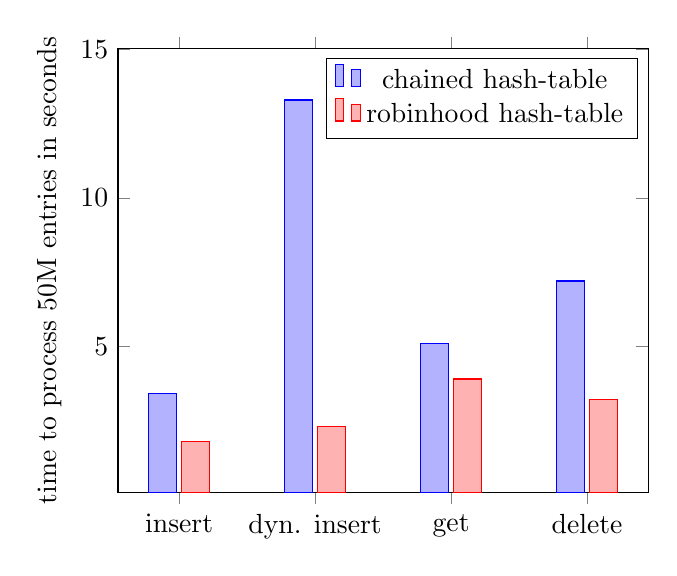
\begin{tikzpicture}
            \begin{axis}[
                scale=0.8,
                ybar,
                %title=\textbf{Chained vs Robinhood Hash-table Performance},
                enlargelimits=0.15,
                % legend style={at={(1.5,-0.15)},
                %   anchor=north,legend columns=-1},
                ylabel={time to process 50M entries in seconds},
                symbolic x coords={insert,dyn. insert,get,delete},
                xtick=data,
                nodes near coords align={vertical},
                ]
            \addplot coordinates {(insert,3.4) (dyn. insert,13.3) (get,5.1) (delete,7.2)};
            \addplot coordinates {(insert,1.8) (dyn. insert,2.3) (get,3.9) (delete,3.2)};
            \legend{chained hash-table, robinhood hash-table}
            \end{axis}
        \end{tikzpicture}
        \caption{Chained vs Robinhood Hash-table Performance}
        \label{fig:ch_vs_rh}
    \end{center}
\end{figure}

\medskip
To see how much better the robinhood hash-table is, we'll benchmark it on four workloads: inserting 50 million entries into a hash-table that has been preallocated to the final size, inserting to an empty hash-table so that it has to dynamically grow, searching for 50 million entries (some of which might not exist), and deleting 50 million entries. We use $50\%$ as a maximum load factor for the robinhood hash-table, although we later lowered this to $20\%$ to increase performance on the leaderboard when it became clear that memory was not a significant concern. See Figure~\ref{fig:ch_vs_rh} for a graph of the results.


\pgfplotstableread{robinhood.dat}{\robinhood}
\pgfplotstableread{robinhood_copy.dat}{\robinhoodcopy}
 \begin{figure}[ht]
     \centering
    \begin{tikzpicture}
        \pgfplotsset{scaled y ticks=false}
    \begin{axis}[
        scale=0.65,
        %ybar,
        %title=\textbf{Chained vs Robinhood Hash-table Performance},
        %enlargelimits=0.15,
        legend style={at={(0.5,-0.25)},
          anchor=north,legend columns=-1},
        grid = both,
        xlabel={entries inserted},
        ylabel={elapsed time in microseconds},
        nodes near coords align={vertical},
    ]
     
    \addplot[red, very thick] table [x = {x}, y = {a}] {\robinhood};
    \addplot[blue, very thick] table [x ={x}, y = {b}] {\robinhood};
    \addplot[green!50!black, very thick] table [x = {x}, y = {c}] {\robinhood};
     
    \legend{
        $50\%$ load,
        $90\%$ load,
        $20\%$ load
    }
     
    \end{axis}
    \end{tikzpicture}~
    \begin{tikzpicture}
        \pgfplotsset{scaled y ticks=false}
    \begin{axis}[
        scale=0.65,
        %ybar,
        %title=\textbf{Chained vs Robinhood Hash-table Performance},
        %enlargelimits=0.15,
        legend style={at={(0.5,-0.25)},
          anchor=north,legend columns=-1},
        grid = both,
        xlabel={entries inserted},
        ylabel={total memory allocated (relative)},
        nodes near coords align={vertical},
    ]
     

    \addplot[blue, very thick] table [x ={x}, y = {y}] {\robinhoodcopy};
     
    \legend{
        $90\%$ load,
    }
     
    \end{axis}
    \end{tikzpicture}
    \caption{Load factor impact on performance of a robinhood hash-table as well as an explanation for the performance jumps}
    \label{fig:load}
 \end{figure}

\medskip
Not only is the robinhood hash-table faster, it is also more memory efficient. Note that with the described load factors, the robinhood hash-table uses only $66\%$ of the memory required by the chained hash-table. If we decrease the max load factor for the robinhood hash-table, we could get even better times. To see how significantly performance is impacted by the maximum load factor, see Figure~\ref{fig:load}. Notice also that there is a slight curve in the $90\%$ load factor graph as the table becomes full. This shape can be explained mathematically as the increasing variance in probe search length as the table becomes increasingly clustered.

 \medskip
 Each of these dips is explained in the second chart of Figure~\ref{fig:load} as the cost of resizing the hash table when the number of entries inserted passes a certain threshold. The optimal solution seems to be to start with a high load factor when the hash-table is small and begin to lower it as the number of elements grows. We didn't explore this dynamic load factor approach in our project.

\subsection{Thread Pool}
\label{threadpool}

Lastly, many tasks in the project require multithreading. To add support for multithreading without too much hassle, we implement an abstraction over threads known as a \textit{thread pool}. When we initialize a \texttt{thread\_pool} struct, it creates an array of threads; for performance reasons usually we make two threads for each logical processor. We use the \texttt{sysconf} call to get the number of logical processors available on the system.

\medskip
The thread pool then has two methods which can be used: \texttt{add\_task\_thread\_pool} and \texttt{wait\_thread\_pool}. The task adding method takes in a function to execute and adds it to a work queue. Once a thread becomes available, it executes the function. The wait method blocks the calling thread until the thread pool has completed all the tasks in the queue. This structure fully avoids race conditions by using a thread-safe linked list for the work queue. 

\medskip
We found that this is a mostly zero-cost abstraction, and that the added flexibility of submitting work chunks without worrying about thread safety outweighed the potential performance increases we would see from custom designing a multithreaded setup for every scenario.

\section{Conclusion}

Having looked at this project's position on the class performance leaderboard, we can safely say that this is a well optimized database management system. (at least by the standards of the class) Our system is especially optimized for loading csv files, performing batched queries, and is very fast at loads. However, it struggles a bit compared to other projects in the class on loading and using indices to speed up selections. This quality in performance of certain areas turned to be roughly proportional to the time spent on each of the areas, so we're sure that given more time we could bring the performance up significantly.

\subsection{Benchmarking Methodology}

In this section we'll describe our methodology for benchmarking. To help with benchmarking, we created a \texttt{globals.h} file which contains many tuning parameters and algorithm selection to make it very easy to quickly switch out different algorithms. For example, the heuristic used for shared scans is stored in this file. We also introduce the \texttt{time()} command in the query language which can be used to time segments of query language code and print the results. This allowed us to generate queries that generate lots of accurate timing results, and this helped remove manual labor for benchmarking. With these tools, it was very easy to write scripts that automated many of the testing procedures in the project.

\medskip
All of the benchmarks were run on a laptop with a 2.3 GHz 8-Core Intel Core i9 processor and 16 GB 2667 MHz DDR4 memory, running a very stripped down version of Arch Linux. We made sure to run each experiment twice and only record the second run to avoid cold cache misses. For cases when there is a lot of noise in the data, we run multiple trials and average the results together. Most of the testing data and queries, especially for large figures such as in Figure~\ref{fig:heuristic} were generated using Python. All the data generated for the database took on a uniform distribution, usually distributed in such a way as to avoid too many duplicate values. It would be interesting to see if a skewed distribution would affect any of the results in this paper, but we did not conduct such experiments.

\begin{thebibliography}{9}
    \bibitem{hash}
    Pedro Celis and Per-{\AA}ke Larson and J. Ian Munro (1985) \emph{Robin hood hashing}, 26th Annual Symposium on Foundations of Computer Science, 281-288. 
\end{thebibliography}


\end{document}